\newpage
\section{Results on the Llama Model}
\label{app:other_model}

\begin{table}[ht]
\centering
\caption{
Comparison with other baselines on mathematical reasoning benchmarks using a Llama series model. \method~achieves competitive performance across benchmarks. \textbf{Bold} indicates the best performance and \underline{underline} indicates second-best.
}
\resizebox{0.38\textwidth}{!}{
\begin{tabular}{c c c c c c}
\toprule
\textbf{Benchmark} & \textbf{Metric} & \textbf{KD} & \textbf{GRPO} & \textbf{OPD} & \textbf{\method} \\
\midrule
\multirow{2}{*}{MATH500}
& Avg@8  & 42.60 & \textbf{45.01} & 43.60 & \cellcolor{blue!10}\underline{44.90} \\
& Pass@8 & 65.80 & \underline{66.00} & 64.80 & \cellcolor{blue!10}\textbf{67.20} \\
\addlinespace
\midrule
\multirow{2}{*}{AMC23}
& Avg@8  & 18.43 & \underline{20.31} & 19.06 & \cellcolor{blue!10}\textbf{22.18} \\
& Pass@8 & \textbf{52.50} & \underline{50.00} & 47.50 & \cellcolor{blue!10}\textbf{52.50} \\
\addlinespace
\midrule
\multirow{2}{*}{AIME24}
& Avg@8  & 1.66 & \textbf{2.91} & \underline{2.08} & \cellcolor{blue!10}\textbf{2.91} \\
& Pass@8 & \textbf{13.33} & \underline{10.00} & \underline{10.00} & \cellcolor{blue!10}\textbf{13.33} \\
\addlinespace
\midrule
\multirow{2}{*}{AIME25}
& Avg@8  & \underline{1.25} & \textbf{2.08} & \underline{1.25}  & \cellcolor{blue!10}\textbf{2.08} \\
& Pass@8 & \underline{6.67} & \textbf{10.00} & \underline{6.67} & \cellcolor{blue!10}\textbf{10.00} \\
\bottomrule
\end{tabular}
}
%\vspace{-0.4cm}
\label{tab:llama_model}
\end{table}
{To verify that the proposed \method~is not limited to a specific model family and can operate effectively on other architectures, we conduct additional experiments on the Llama series~\cite{grattafiori2024llama}. Specifically, we use Llama-3.2-3B-Instruct as the student model and Llama-3.1-8B-Instruct as the teacher model, and perform training under the same framework.
The baseline setup follows ~\S\ref{sec:experimental_settings}, including KD, GRPO, and OPD.
Experimental results reported in ~\autoref{tab:llama_model} show that \method~achieves competitive performance compared to other baselines on the Llama model as well, suggesting that \method~can be generally applied.}

{Additionally, we analyze the training dynamics by measuring the forward KL divergence between the teacher and student distributions at token positions where the teacher exhibits high entropy (entropy $\ge 0.8$). As shown in \autoref{fig:llama_fkl}, under OPD, the forward KL remains high in these regions and exhibits substantial fluctuations throughout training. This implies that reverse KL–based reward produces unstable signals in regions where the teacher distribution has high entropy, as observed in the toy experiment in \S\ref{sec:instability}. In contrast, \method~maintains lower forward KL values in the same high-entropy regions and exhibits more stable training behavior, indicating better preservation of the teacher’s distributional structure and uncertainty, which is reflected in the benchmark performance gains.}
\begin{figure}[H]
  \centering
    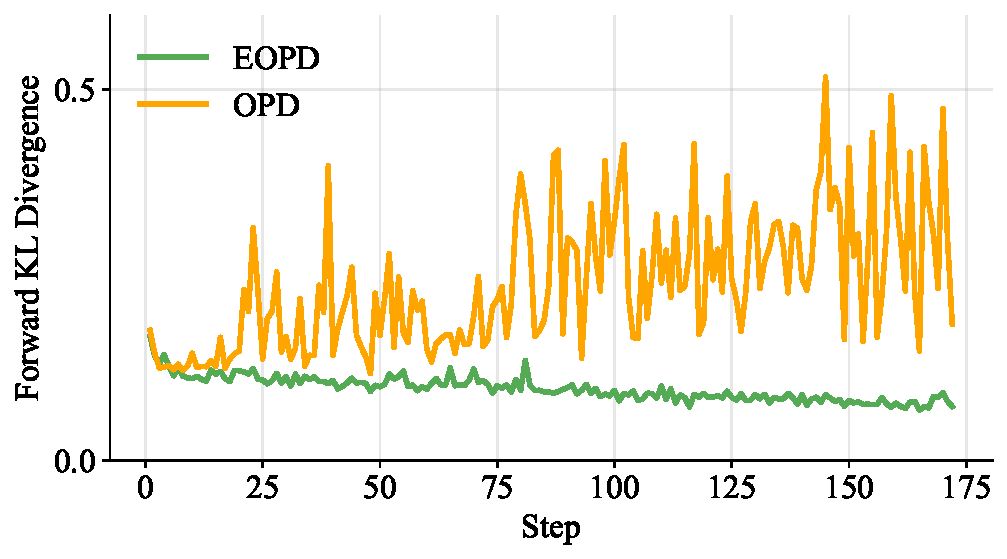
\includegraphics[width=0.5\linewidth]{figure/llama_fkl.pdf}
  \caption{Average forward KL divergence measured during training at token positions where the teacher distribution exhibits high entropy (entropy $\ge 0.8$) for the Llama-3.2-3B-Instruct student.}
  \label{fig:llama_fkl}
\end{figure}
